\documentclass[a4paper,10pt]{article}
\usepackage[utf8]{inputenc}
 
% Blank line between paragraphs instead of indenting the first line
\usepackage{parskip}
\setlength{\parskip}{\baselineskip}

% Squash a bit more text onto a page
\usepackage{geometry}
\geometry{verbose,tmargin=20mm,bmargin=20mm,lmargin=25mm,rmargin=25mm}

% Indent verbatim environments
\catcode`\@=11
\let \saveverbatime \@xverbatim
\def \@xverbatim {\leftskip = 1cm\relax\saveverbatime}
\catcode`\@=12

\usepackage{graphicx}
\usepackage{listings}
\usepackage{amsmath}

\lstdefinelanguage{logicdef}
{
  morekeywords={DEVICES, MONITORS, CONNECTIONS, END},
  sensitive=false,
  morecomment=[s]{/*}{*/},
basicstyle=\small\ttfamily,
keywordstyle=\pmb,
frame=single,
numbers=left,
numberstyle=\tiny
}



\begin{document}

\begin{center}
\LARGE \textbf{IIA GF2 Software: 1st interim report}

\small Team 8 - Martin Jackson (mj380), Tim Hillel (th389) and Jamie Magee (jam96)
\end{center}



\section{Introduction}


\section{General approach}



\section{Syntax and semantics}

\begin{verbatim}
specfile = block {block}
block = devices|connections|monitors
devices = 'DEVICES' dev {';' dev} 'END'
connections = 'CONNECTIONS' con {';' con} 'END' 
monitors = 'MONITORS' mon {';' mon} 'END'
\end{verbatim} 

\textbf{Semantics:} An input file is composed of device, connection and monitor blocks. There must be at least one devices block in the input file. Connection and monitor blocks may be omitted. There may be more than one of each type of block. 

\begin{verbatim}
dev = clock|switch|gate|dtype|xor
clock = 'CLOCK' devicename':'digit{digit}
switch = 'SWITCH' devicename':'('0'|'1')
gate = ('AND'|'NAND'|'OR'|'NOR') devicename':'('1'|'2'|'3'|'4'|'5'|'6'|
       '7'|'8'|'9'|'10'|'11'|'12'|'13'|'14'|'15'|'16')
dtype = 'DTYPE' devicename
xor = 'XOR' devicename
\end{verbatim} 

\textbf{Semantics:} These statements define a new device of the specified type. Multiple devices may not be defined with the same \texttt{devicename}. Each \texttt{devicename} must be defined in a devices block before being referred to in a connections or monitors block. \texttt{devicename} is case sensitive. For a \texttt{CLOCK}, the integer parameter must be greater than zero. For \texttt{SWITCH} devices, the parameter is the initial state of the device (1 is on, 0 is off). For logic gates (\texttt{AND}, \texttt{NAND}, \texttt{OR}, \texttt{NOR}), it is the number of inputs.

\begin{verbatim}
con = devicename['.'input] '=' devicename['.'output]
\end{verbatim} 
\textbf{Semantics:} Connects the specified device input to the specified device output. Multiple inputs may be connected to the same output, but attempting to connect multiple outputs to the same input is a semantic error. All inputs must be connected. 

\begin{verbatim}
mon = devicename['.'output]
\end{verbatim} 
\textbf{Semantics:} Adds an output signal to the list of signals to be monitored. Duplicate monitor statements for the same output signal are ignored. 

\begin{verbatim}
devicename = letter {letter|digit}
input = 'I'('1'|'2'|'3'|'4'|'5'|'6'|'7'|'8'|'9'|'10'|'11'|'12'|'13'|'14'|
        '15'|'16')|'DATA'|'CLK'|'SET'|'CLEAR'
output = 'Q'['BAR']
\end{verbatim} 

\verb|devicename['.'input]| indicates an input pin on a device. If the device has multiple input pins, the input pin name must be given. If the device has a single input that has a name (such as a 1 input logic gate with input \texttt{I1}), then the input pin name is optional and defaults to the single input. If the inputs do not have names, the input pin name must be omitted.
The input pin must be valid according to the properties of the device that \texttt{devicename} refers to. For example, for a gate defined to have 4 inputs, only \texttt{I1}, \texttt{I2}, \texttt{I3}, and \texttt{I4} may be used; and \texttt{DATA}, \texttt{CLK}, \texttt{SET}, and \texttt{CLEAR} may only be used when \texttt{devicename} is a \texttt{DTYPE}.

\verb|devicename['.'output]| indicates an output pin on a device. \texttt{output} must be a valid output for the type of device that \texttt{devicename} refers to. If the device has multiple outputs, \texttt{output} must be given, otherwise it must be omitted. 

\texttt{DEVICES}, \texttt{CONNECTIONS}, \texttt{MONITORS}, and \texttt{END} are reserved words, and must not be used as device names.

Comments start with \texttt{/*} and are terminated by the first \texttt{*/}. A \texttt{/*} inside a comment is ignored. 

\section{Error handling}

\subsection{Syntax errors}

If a semicolon is omitted, an error message should be printed and text should be skipped until the next semicolon is found. Scanning should then continue as normal.

If a \texttt{dev}, \texttt{con}, or \texttt{mon} statement does not conform to the correct syntax, then it will be ignored, an error message will be printed, and scanning will continue after the next semicolon. 

If statements are present outside a devices, connections, or monitors block, then an error message will be printed and they will be ignored. Scanning will continue at the next \texttt{DEVICES}, \texttt{CONNECTIONS}, or \texttt{MONITORS} keyword. 

If \texttt{DEVICES}, \texttt{CONNECTIONS}, or \texttt{MONITORS} keyword appears without using \texttt{END} to terminate the previous block, an error message will be printed and scanning will continue as though the previous block was correctly terminated. 

If a comment is not terminated before the end of the file, then an error message will be printed. The contents of the comment will still be ignored. 

For all syntax errors, the error message will include the line number and indicate the position on that line of the error.


\subsection{Semantic errors}

Semantic errors in a \texttt{dev}, \texttt{con}, or \texttt{mon} statement will cause an error message to be printed with details about which semantic rule has been broken, and that statement will be ignored. 

\clearpage
\appendix

\section{Appendix: Gantt chart}
\begin{figure}[h]
 \centering
  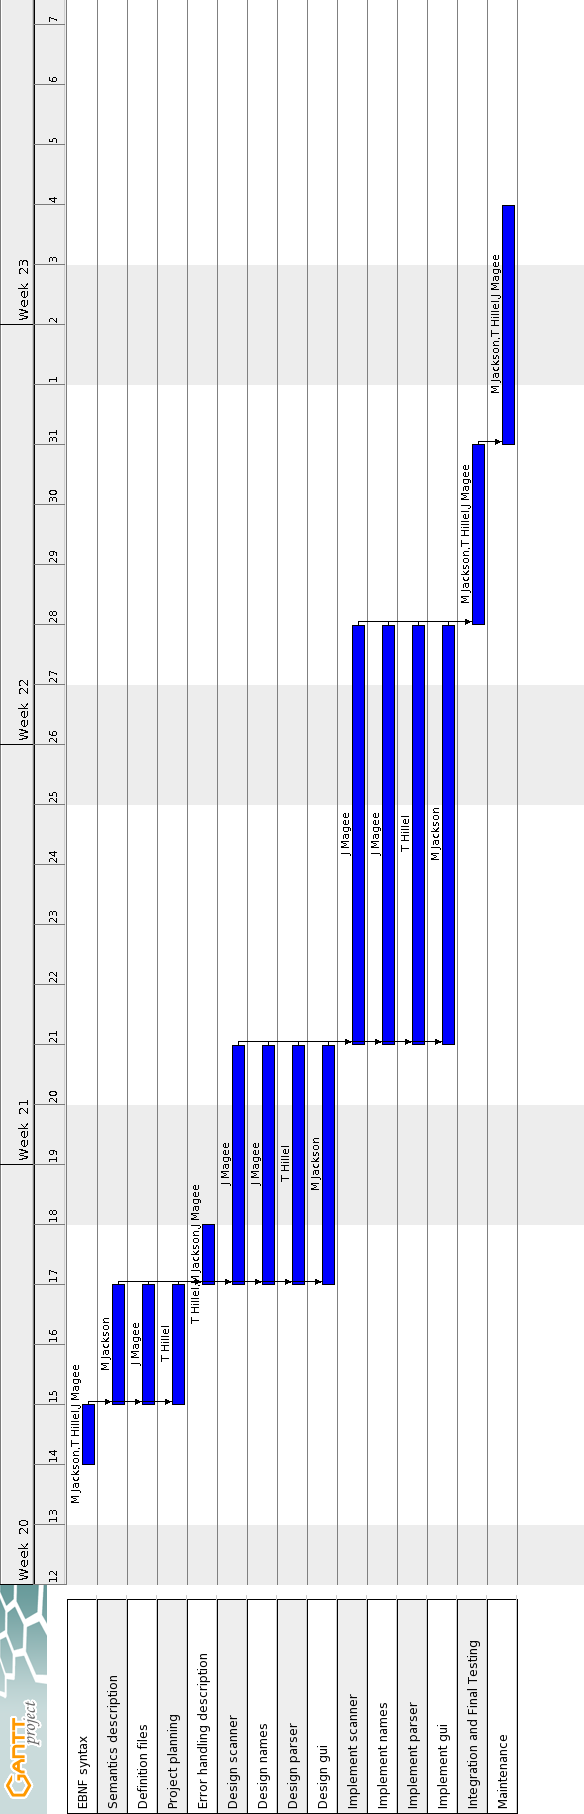
\includegraphics[height=19cm]{../../Common/Gantt-Chart.png}
 \caption{Gantt chart showing key events in development cycle}
 \label{fig:ganttchart}
\end{figure}

\clearpage

\section{Appendix: examples}

\subsection{Example circuit diagrams}
\begin{figure}[h]
 \centering
 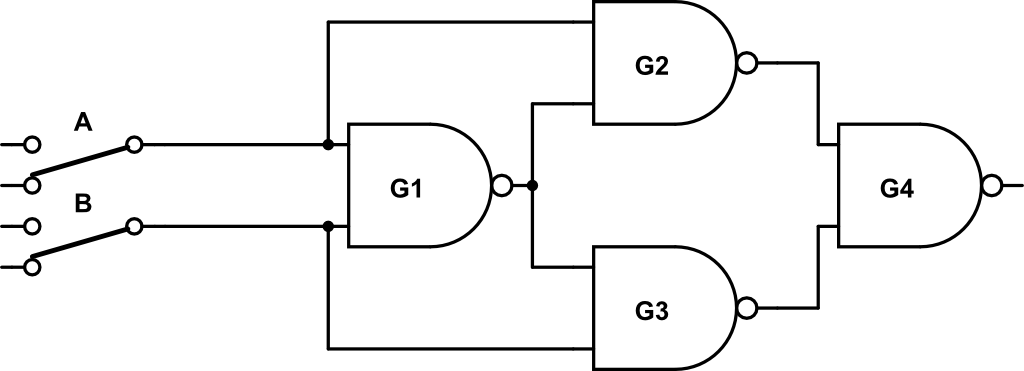
\includegraphics[width=14cm]{../../jam96/xor.png}
 \caption{Circuit diagram of an XOR gate implemented using NAND gates}
 \label{fig:example-xor}
\end{figure}

\begin{figure}[h]
 \centering
 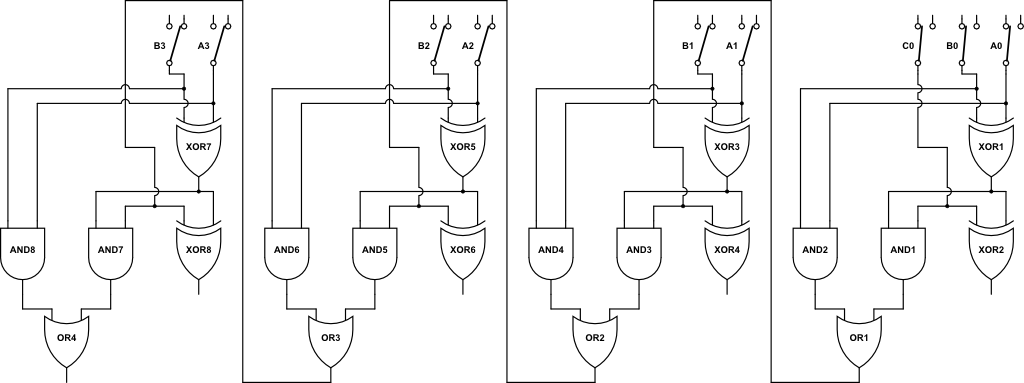
\includegraphics[width=16cm]{../../jam96/4-bit-adder.png}
 \caption{Circuit diagram of a 4 bit adder}
 \label{fig:example-adder}
\end{figure}


\subsection{Example definition file for XOR gate circuit}
\lstinputlisting[language=logicdef]{../../jam96/xor.txt}

\subsection{Example definition file for 4 bit adder circuit}
\lstinputlisting[language=logicdef]{../../jam96/4bitadder.txt}

\end{document}


